\documentclass[12pt,letterpaper]{article}

\usepackage{amsmath, amsthm}
\usepackage{microtype, parskip}
\usepackage[comma,numbers,sort&compress]{natbib}
\usepackage{lineno}
\usepackage{docmute}
\usepackage{caption, subcaption, multirow, morefloats, rotating}
\usepackage{wrapfig}
\usepackage{attrib}

\frenchspacing

\begin{document}

\section*{Introduction}
Changes to species diversity are the result of evolutionary and ecological processes acting both in concert and continually. Local communities are shaped by dispersal and local ecological processes such as resource competition and predator-prey relationships. The constituent species of these community are drawn from a regional species pool, or the set of all species that are present in at least one community within a region \citep{Mittelbach2015a,Urban2008,Harrison2008}. Species dispersal from the regional species pool to the local communities is a sorting process shaped by biotic and abiotic environmental filters which are mediated by those species' traits \citep{Shipley2006,Elith2009,Urban2008,Loeuille2008,Cottenie2005,Harrison2008}. Regional species pools are shaped by speciation, extinction, migration, and extirpation. The gain or loss of regional diversity is the result of macroevolutionary dynamics which, in turn, shape the downstream macroecological dynamics of the regional species pool and its constituent local communities \citep{Urban2008,Mittelbach2015a,Harrison2008}. 

Fundamentally, all species respond differently to climate and environmental change \citep{Blois2009}. Similarities in ecological roles of species within a regional species pool can be described as a collection of guilds or functional groups \citep{Valentine1969,Bambach1977,Brown1989,Simberloff1991a,Wilson1999}. Species within the same functional group are expected to have more similar macroecological dynamics to each other than to species of a different functional group. By focusing on the relative diversity of functional groups, changes to diversity are interpretable as changes to the set of ways species within a species pool could interact with the biotic and abiotic environment. 

A key question when comparing communities or regional species pools based on their functional composition is whether specific functional groups are enriched or depleted and why; what are the processes that led to a species pool having the functional composition it does \citep{Mcgill2006,Weber2017,Brown1989,Smith2008b,Blois2009}? Comparisons of contemporaneous regional species pools only determines if a functional group is enriched or depleted in one species pool relative to other species pools. This type of comparison does not reveal if that functional group is enriched or depleted relative to its diversity in the regional species pool over time \citep{Blois2009}. While a species pool may be depleted of a functional group relative to other contemporaneous species pools, that same functional group may be actually be enriched in that species pool relative to its historical diversity. Because the processes which shape regional species pool diversity (e.g. origination, extinction) operate on much longer time scales than is possible for studies of the Recent, paleontological data provides a unique opportunity to observe and estimate the changes to functional diversity and how species functional traits and environmental context can shape the enrichment or depletion of functional groups within a regional species pool \citep{Blois2009,Smith2008b}. Being able to identify which if the diversity of any functional groups are depleted relative to their long term average diversity in the species pool is particularity useful in conservation settings; species in depleted groups are most likely more at risk of extinction than species in enriched groups, even if those enriched groups are relatively rare when compared to the functional composition of other contemporaneous species pools.

The paleontological record of North American mammals for the Cenozoic (\(\sim\) 66 million years ago to present) provides one of the best opportunities for understanding how regional species pool functional diversity changes over time. The North American mammal record is a relatively complete temporal sequence for the entire Cenozoic which primarily, but not exclusively, based on fossil localities from the Western Interior of North America \citep{Alroy1996a,Alroy2000g,Alroy2009}. Additionally, mammal fossils preserve a lot of important physiological information, such as teeth, so that functional traits like the dietary/trophic category of species are easy to estimate \citep{Polly2015a,Polly2011b,Eronen2010a}.

The goals of this study are to understand when are unique functional groups, called ecotypes, enriched or depleted in the North American mammal regional species pool and to estimate the relationship between changes to regional ecotypic diversity and changes to their environmental context.

\subsection*{Background}

The diversity history of North American mammals for the Cenozoic is relatively well understood as it has been the focus of considerable study \citep{Alroy2009,Alroy1996a,Janis1993b,Alroy2000g,Figueirido2012,Pires2015a,Fraser2015a,Smits2015b,Quental2013,Slater2015c,Silvestro2015b,Badgley2013,Blois2009,Janis1993c}. Previous approaches to understanding mammal diversity, both in North America and elsewhere, fall into a number of overlapping categories: total diversity \citep{Alroy2000g,Alroy1996a,Figueirido2012,Liow2008}, with/between guild comparisons \citep{Janis2004,Janis2000,Jernvall2004,Janis1993c,Pires2015a,Janis2008a}, within/between clade comparisons \citep{Quental2013,Slater2015c,Silvestro2015b,Fraser2015a,Cantalapiedra2017}, and estimating the impact of environmental process on diversity \citep{Blois2009,Janis1993c,Janis1993b,Fraser2015a,Eronen2015,Badgley2013,Badgley2017,Alroy2000g}. Each of these individual perspectives provide a limited perspective on the macroevolutionary and macroecological processes shaping diversity and diversification. Integration across perspectives is necessary for producing a holistic and internally consistent picture of how the North American mammal species pool has changed through time. One of the goals of this study is to present a framework for approaching hypotheses about diversity and diversification through multiple lenses simultaneously so that our inferences are better constrained and the relative importance of various functional traits and environmental factors may be better elucidated.

The narrative of the diversification of North American mammals over the Cenozoic is one of gradual change. There is little convincing evidence that there have been any major or sudden cross-functional group or cross-taxonomic turnover events in mammal diversity at any point in the Cenozoic record of North America \citep{Alroy2009,Alroy1996a,Eronen2015,Janis1993b,Alroy2000g}. Instead of being concentrated at specific time intervals, species turnover has been found to be distributed through time. It is then expected then that, for this analysis, turnover events or periods of rapid diversification or depletion should not occur simultaneously for all functional groups under study. Additionally, changes to mammal diversification seem to be primarily driven by changes to origination rate and not to extinction \citep{Alroy1996a,Alroy2000g,Alroy2009}. An unresolved aspect of the general history of mammal diversification is whether that diversity is limited or self-regulating; namely, to what extent is mammal diversification diversity-dependent \citep{Alroy2009,Rabosky2015b,Harmon2015a,Rabosky2013a}. Similarity, this question can also be asked of specific functional groups \citep{Jernvall2004,Valkenburgh1999,Silvestro2015b,Quental2013}.

Within the overall narrative of mammal diversity, the histories of a selection of taxonomic and functional groups are better understood. These groups have particularity good fossil records and/or have been the focus of previous analyses.

The diversity history of ungulate herbivores has been characterized by more recently originating taxa having longer legs, higher crowned teeth, and a shift from graze-dominated to browse-dominated diets than their earlier originating counterparts \citep{Janis2004,Janis2000,Janis1993b,Janis2008a,Cantalapiedra2017,Fraser2015a}. The mechanisms which drive this pattern are theorized to be some combination of tectonic activity driving environmental change such as the drying of the western interior of North America due mountain building and global temperature and environmental change such as the formation of polar icecaps \citep{Janis2008a,Eronen2015,Blois2009,Badgley2017}. 

In contrast, the origination of modern cursorial carnivore forms was not until later in the Cenozoic; this is not to say that carnivore diversity only grew in the late Cenozoic, but that those forms were late entrants \citep{Janis1993c}. Instead, the diversity history of carnivores is reflective of density-dependence or some other form of self-regulation \citep{Valkenburgh1999,Silvestro2015b,Slater2015c}. Specifically, it has been proposed that different canid clades have replaced each other as the dominate members of their functional group within the species pool \citep{Silvestro2015b,Valkenburgh1999}. It is then expected that, for this analysis, the diversity of digitigrade and plantigrade carnivores (i.e. the ``carnivore'' guild of \citet{Valkenburgh1999}) should be relatively constant for the Cenozoic or at least have plateaued by the Neogene.

In a relevant study, \citet{Smits2015b} found that functional traits such as a species dietary or locomotor category structure differences in mammal extinction risk. In particular, arborel taxa were found to have a shorter duration on average than species from other locomotor categories \citep{Smits2015b}. Two possible scenarios that could yield this pattern were proposed: the extinction risk faced by arboreal species is constant and high for the entire Cenozoic or the Paleogene and Neogene represent different regimes and extinction risk increased in the Neogene, thus driving up the Cenozoic average extinction risk. These two possible explanations have clear and testable predictions with respect to the diversity history of arboreal taxa: 1) if arboreal taxa always have an elevated extinction risk when compared to other taxa, then the diversity history of arboreal taxa is expected to be constant with time, albeit possibly at low diversity; and 2) if the Paleogene and Neogene represent difference selective regimes with the former being associated with lower extinction risk than the latter, then the diversity history of arboreal taxa are expected to be present in the Paleogene but depleted or absent from the species pool during the Neogene.

%There is some uncertainty and a lack of consensus as to the effect of species body size on mammal diversity and aspects of the diversification processes, specifically extinction \citep{Liow2008,Liow2009,Tomiya2013,Smits2015b}. Species body size is frequently framed as an important biological descriptor because of its correlation with other important and relevant ecological traits such as metabolic rate and home range size \citep{Brown1995}. It is also relatively easy to estimate for extinct species using proxy measures and regression equations, as was done in this study (see below). However, body size is normally analyzed without simultaneous reference to other species traits \citep{Liow2008,Huang2017,Raia2012f,Smith2004}, but see \citep{Smits2015b}; this combined with the high amount of correlation between life history traits and body size limits processed-based inference, because the actual causal mechanisms underlying an observed pattern are obscured or missing.

The climate history of the Cenozoic can be broadly described as a gradual cooling trend, with polar ice-caps forming in the Neogene \citep{Zachos2001,Zachos2008,Cramer2011}. There are of course exceptions to this pattern such as the Eocene climatic optimum, the mid-Miocene climatic optimum, and the sudden drop in temperature at the Eocene/Oligocene boundary \citep{Zachos2001,Zachos2008}. In terms of the North American biotic environment, the Cenozoic is additionally characterized by major transition from having closed, partially forested biomes being common in the Paleogene to the landscape being dominated by savannah and grasslands biomes by the Neogene \citep{Blois2009,Janis1993b,Janis2000,Stromberg2005}. Additionally, the landscape structure and topology of North America changed substantially over the Cenozoic with mountain uplift and other tectonic actives in Western North America \citep{Blois2009,Eronen2015,Janis2008a,Badgley2013}. This type of geological activity affects both local climates as well as continental weather patterns while also mobilizing increased grit into the environment, something which may be responsible for increasing trend of hyposodony (high crowned teeth) among herbivores \citep{Jardine2012,Jernvall2002,Damuth2011}.

%The Eocene-Oligocene transition has been observed to be associated with extinction of many ungulate taxa \citep{Janis2008a}. This boundary also marks the transition from the Paleogene to the Neogene and from herbivores being browsing dominated to grazing dominated, though not concurrently \citep{Janis1993b,Stromberg2005}. Additionally, the Paleogene-Neogene boundary marks the approximate start of Antarctic ice sheets, which were previously absent \citep{Zachos2008}. There is an observed stability in estimates of global temperature from the E/O transition till the end of the Miocene called the Mid-Miocene climatic optimum \citep{Zachos2001,Zachos2008}. The Mid-Miocene climatic optimum is bookended by periods of temperature decline. We would then expect that, for the Miocene, turnover and other diversification events would most likely be due to biological interactions or immigration and not biotic-abiotic interactions because of the constancy of the climate, and that those groups that are driven primarily by environmental factors, the Miocene would be a period of marked by an absence of major changes to diversity or the diversification process.

The effect of climate on mammal diversity and its accompanying diversification process has been the focus of considerable research with a slight consensus favoring mammal diversification being more biologically-mediated than climate-mediated \citep{Alroy2000g,Figueirido2012,Clyde1998a}. However, differences in temporal and geographic scale seem to underly the contrast between these two perspectives. For example when the mammal fossil record analyzed at small temporal and geographic scales a correlation between diversity and climate is observable \citep{Clyde1998a}. However, when the record is analyzed at the scale of the continent and most of the Cenozoic this correlation disappears \citep{Alroy2000g}. This result, however, does not go against the idea that there may be short periods of correlation between diversity and climate and that this relationship can change or even reverse direction over time; this type result means that there is no single direction of correlation between diversity and climate \citep{Figueirido2012}. 

In the case of a fluctuating correlation between diversity and climate it is hard to make the argument for an actual causal link between the two without modeling the underlying ecological differences between species; after all, species respond differently based on their individual ecologies \citep{Blois2009}. When analysis is based on diversity or taxonomy alone no mechanisms are possible to infer. Taxonomy, like body size, stands in for many important species traits to the point that mechanistic or process based inference is impossible. While emergent patterns might correspond to taxonomic grouping, this itself is an emergent phenomenon. Instead, by framing hypotheses in terms of species traits and their environmental context, these emergent phenomena can be observed and analyzed rather than assumed.



\subsection*{Foreground}

Fourth-corner modeling is an approach to explaining the patterns of either species abundance or presence/absence in a community as a product of species traits, environmental factors, and the interaction between traits and environment \citep{Brown2014c,Warton2015a,Pollock2012,Jamil2013}; effectively uniting climate-based species distribution modeling (SDMs) with trait-based community assembly models (CATS, MaxEnt). In modern ecological studies, what is being modeled is species occurrences at localities distributed across a region \citep{Pollock2012,Jamil2013}. In this study, what is being modeled is the pattern of species occurrence over time for most of the Cenozoic record for North America (Fig. \ref{fig:concept_fourth_corner}). By analyzing assemblages over time instead of space in fourth-corner framework we can gain better inference of how an instantaneous species pool (i.e. the Recent) is assembled over time. These two approaches, modern and palentologicial, are different views of the same three-dimensional pattern: species at localities over time. The temporal limitations of modern ecological studies and difficulties with uneven spatial occurrences of fossils in paleontological studies means that these approaches are complementary and reveal different patterns of how species are distributed in time and space.

\begin{figure}[ht]
  \centering
  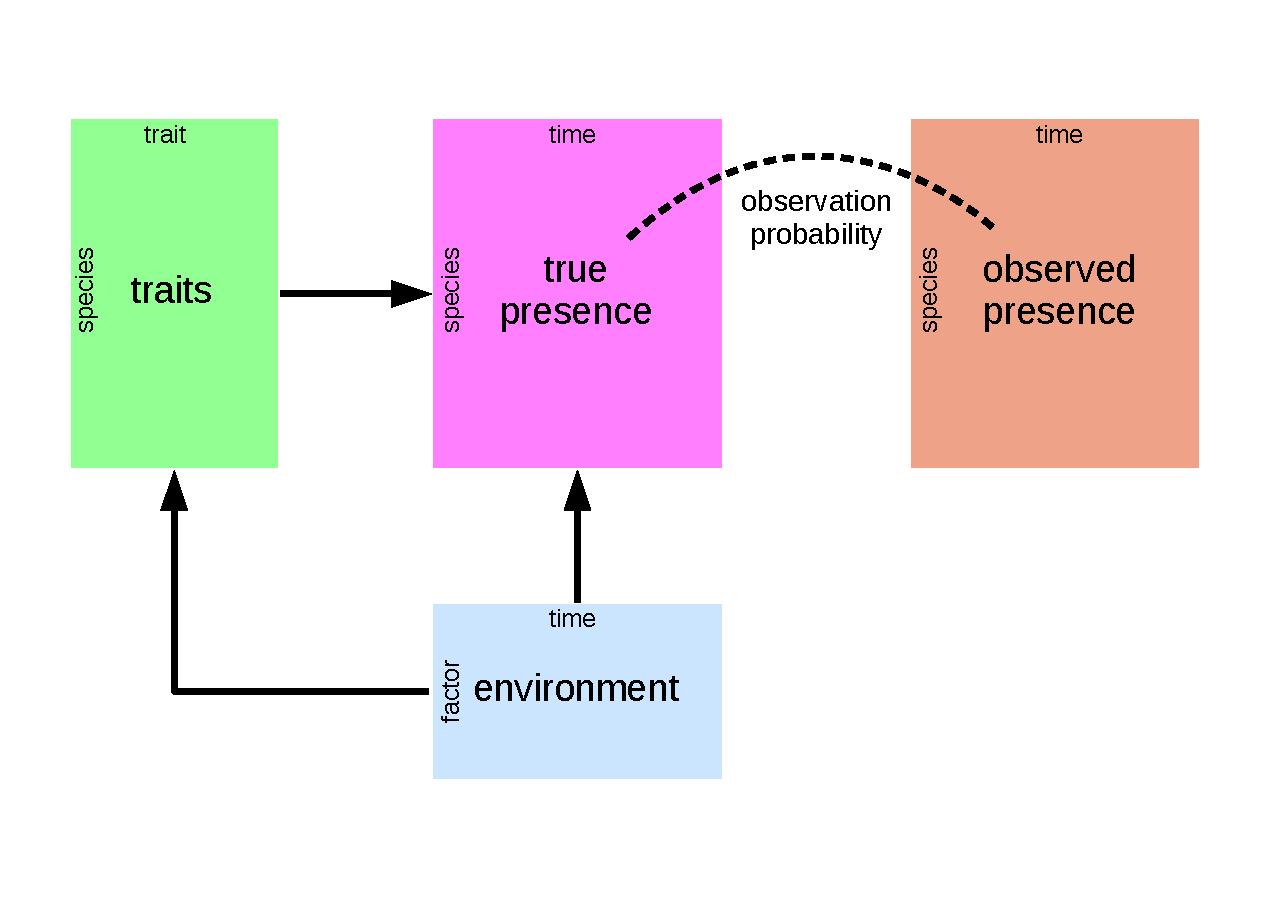
\includegraphics[width=\textwidth,height=0.4\textheight,keepaspectratio=true]{figure/paleo_fourth_corner}
  \caption[Conceptual diagram of the paleontological fourth-courner problem]{Conceptual diagram of the paleontological fourth corner problem. The observed presence matrix (orange) is the empirical presence/absence pattern for all species for all time points; this matrix is an incomplete observation of the ``true'' presence/absence pattern (purple). The estimated true presence matrix is modeled as a function of both environmental factors over time (blue) and multiple species traits (green). Additionally, the effects of environmental factors on species traits are also modeled, as traits are expected to mediate the effects of a species environmental context. This diagram is based partially on material presented in \citet{Brown2014c} and \citet{Warton2015a}.}
  \label{fig:concept_fourth_corner}
\end{figure}

My approach to delimiting and assigning mammal functional groups is inspired on the ecocube heuristic used to classify marine invertebrate species by three functional traits \citep{Bush2007,Bambach2007,Bush2011,Bush2012b,Novack-Gottshall2007,Villeger2011}. Unique combinations of traits represent ecotypes, which are equivalent to functional groups defined by species functional traits instead of a holistic understanding how a taxon interacts with its environment. In this study, the two functional traits used to define a species' ecotype are dietary (e.g. herbivore, carnivore, etc.) and locomotor category (e.g. arboreal, unguligrade, etc.). Species body mass was also included as a species trait in this analysis, but not as a functional trait for defining ecotypes; instead, its inclusion is principally to control for differences in species dynamics that driven by mass and not ecotype.

The environmental factors included in this study are estimates of global temperature and the changing floral groups present in North America across the Cenozoic \citep{Cramer2011,Graham2011a}. These covariates were chosen because they provide high level characterizations of the environmental context of the entire North American regional species pool for most of the Cenozoic. Importantly, the effects of a species ecotype on diversity are themselves modeled as functions of environmental factors (Fig. \ref{fig:concept_fourth_corner}) allowing for inference as to how a species ecology can mediate selective pressures do to its environmental context. 

All observations, paleontological or modern, are made with uncertainty. With presence/absence data this uncertainty comes from not knowing if an absence is a ``true'' absence or just a failure to observe \citep{Royle2008,Royle2005,Foote1999a,Foote2001,Lloyd2011,Wang2016b}. For paleontological data, the incomplete preservation and sampling of species means that the true times of origination or extinction may not be observed \citep{Foote1999a,Foote2001,Wang2015,Wang2016b}. The model(s) I propose below represent an attempt to translate the verbal/visual model described here (Fig. \ref{fig:concept_fourth_corner}) into a statistical model for estimating the relative diversity of mammal ecotypes over time and how those ecotypes respond to changes to environmental context while taking into account the fundamental incompleteness of the fossil record.

Ultimately, the goals of this analysis are to understand when are different ecotypes enriched or depleted in the North American mammal regional species pool and how these changes in ecotypic diversity are related to changes in species' environmental context. In the analyses done here, many covariates which describe a species' macroecology and its environmental context are considered. In order to analyze this complex and highly structured data set, I developed a hierarchal Bayesian model combing the fourth-corner modeling approach with a model of an observation-occurrence or observation-origination-extinction process. %The complexity and nuance inherent in questions that are focus of this study, it is possible to consider and test a large number of possible hypotheses. The hierarchical Bayesian modeling approach used here is appropriate for mitigating complications arising from both this complexity and the plethora of testable hypotheses (e.g. multiple comparisons, garden of forking paths) \citep{Gelman2013d,Gelman2012a,Gelman2014}.


\end{document}
